\documentclass[11pt, a4paper]{article}

\usepackage{fontspec}
\usepackage{ucharclasses}
\usepackage{graphicx}
\usepackage{booktabs}
\usepackage{float}
\usepackage{amsmath}
\usepackage{amssymb}
\usepackage{hyperref}
\usepackage{geometry}
\usepackage{caption}

\geometry{a4paper, left=2.5cm, right=2.5cm, top=2.5cm, bottom=2.5cm}

% Typography
\setlength{\parskip}{0.45em}
\setlength{\parindent}{2em}
\linespread{1.25}
\emergencystretch=2em

\setmainfont{Palatino}
\setsansfont{Helvetica Neue}
\setmonofont{Menlo}[Scale=0.88]

\newfontfamily\zhfont{Songti SC}[BoldFont=Heiti SC, Scale=1.02]
\setTransitionsForChinese{\zhfont}{}

\XeTeXlinebreaklocale "zh"
\XeTeXlinebreakskip = 0pt plus 1pt minus 0.1pt

\hypersetup{
    colorlinks=true,
    linkcolor=black,
    citecolor=black,
    urlcolor=blue
}

\captionsetup{font=small, labelfont=bf}

% Section spacing, consistent with the HW1 report style.
\makeatletter
\renewcommand\section{\@startsection{section}{1}{\z@}{-1.2em \@plus -0.3em}{0.5em}{\normalfont\Large\bfseries}}
\renewcommand\subsection{\@startsection{subsection}{2}{\z@}{-0.9em \@plus -0.2em}{0.3em}{\normalfont\large\bfseries}}
\renewcommand\subsubsection{\@startsection{subsubsection}{3}{\z@}{-0.6em \@plus -0.2em}{0.2em}{\normalfont\normalsize\bfseries}}
\makeatother

\title{\textbf{PJ-AG4 项目中期报告}\\[0.35em]
{\large LLM 驱动的高端 GPU 算力现货市场多 Agent 博弈仿真}}
\author{易俊融}
\date{\today}

\begin{document}
\maketitle
\vspace{-1em}

\begin{abstract}
\noindent
本项目构建一个面向高端 GPU 算力现货与供应链分销市场的多 Agent 动态博弈仿真系统。市场中包含规模主导型 Hyperscaler、稳健交付型 PremiumCloud 和现货套利型 SpotBroker 三类异质 Agent。每个 Agent 在有限历史信息下进行需求预测、报价和新增供给决策，环境根据价格、品牌、声誉、库存、缺货和同行算力拆借机制完成统一结算。中期阶段已经完成可复现仿真内核、LLM 决策后端、启发式回退策略、CSV/PDF/HTML 输出和量化实验工具。本报告以本地 OpenAI-compatible 端点接入的 LLM 20 轮实验为主，结果显示 LLM 策略在 seed=7 的实验中达到 0.9963 的市场履约率和 1010.34 的市场总利润，相比同设置启发式基线在总利润上更高，但伴随 Hyperscaler 的轻微缺货和一次 default 事件。实验表明，声誉约束、价格纪律和库存控制共同塑造了 Agent 间的收益分化，项目已经具备进入最终实验扩展和论文式分析的基础。

\vspace{0.4em}
\noindent\textbf{关键词：} 多 Agent 仿真；大语言模型；市场博弈；GPU 算力；声誉机制；供应链
\end{abstract}

%=============================================
\section{引言}

高端 GPU 算力市场同时具有金融现货市场、供应链分销市场和云资源调度市场的特征。一方面，训练与推理需求受到大模型发布、企业采购周期、算力集群扩容和外部冲击影响，呈现明显的时间波动；另一方面，高端 GPU 节点又具有重资产属性，未售出或未出租的算力会持续产生托管、电力、资金占用和技术折旧成本。供应商不仅需要制定价格，还需要决定备货规模、履约优先级和同行间临时拆借策略。

本项目以该场景为背景，研究由 LLM Agent 参与的重复市场博弈。与静态定价模型不同，本项目关注三个问题：第一，不同经营风格的 Agent 在重复竞争中的收益差异如何形成；第二，有限理性和带噪声需求观察如何影响 Agent 的预测与库存决策；第三，声誉机制能否约束低价倾销、违约和拒绝合作等短期行为。

中期阶段的目标不是完成真实市场预测系统，而是完成一个规则透明、可复现、可替换策略后端的实验平台。当前项目已经实现从场景设计到可运行系统的闭环，并能够使用本地 OpenAI-compatible LLM 端点直接生成 Agent 决策。本报告总结系统建模、代码实现、LLM 实验结果、当前不足和后续计划。

%=============================================
\section{市场模型与机制设计}

\subsection{Agent 角色设定}

市场中包含三个独立决策者，分别代表高端 GPU 算力市场中的三类典型经营主体。表~\ref{tab:agents} 总结了其角色差异。

\begin{table}[H]
\centering
\caption{三类市场参与者设定}\label{tab:agents}
\vspace{0.3em}
\begin{tabular}{@{}llll@{}}
\toprule
Agent & 角色定位 & 决策倾向 & 主要风险 \\
\midrule
Hyperscaler & 规模主导型供应商 & 低价、大容量、争夺份额 & 价格战与利润侵蚀 \\
PremiumCloud & 稳健交付型云服务商 & 高声誉、SLA、价格纪律 & 高价下份额流失 \\
SpotBroker & 现货套利型经纪商 & 灵活调价、轻库存、高周转 & 缺货与长期声誉不足 \\
\bottomrule
\end{tabular}
\end{table}

每一轮 $t$ 中，Agent $i$ 选择报价 $p_{i,t}$ 和新增可交付节点数 $q_{i,t}$。轮初库存为 $I_{i,t}$，因此本轮可用供给为
\[
A_{i,t}=I_{i,t}+q_{i,t}.
\]

\subsection{动态需求与有限理性观察}

市场总需求由趋势、季节项、冲击项和自回归噪声构成：
\[
D_t = \max\{D_{\min},\ b + gt + S_t + H_t + \epsilon_t\}.
\]
其中 $b$ 为基准需求，$g$ 为趋势增长率，$S_t$ 为周期项，$H_t$ 为外部冲击，$\epsilon_t$ 为 AR 噪声。Agent 不能直接观察完整真实需求，而是接收带噪声的观测需求和有限窗口历史。这一设计用于刻画现实市场中的信息不完全和有限理性。

\subsection{需求分配、拆借与收益结算}

需求分配采用 logit 型吸引力机制。Agent 的市场吸引力为
\[
a_{i,t}=b_i+\beta_R R_{i,t}-\beta_p p_{i,t},
\]
其中 $b_i$ 是品牌强度，$R_{i,t}$ 是声誉，$\beta_R$ 和 $\beta_p$ 分别表示声誉权重和价格敏感度。需求份额为
\[
s_{i,t}=\frac{\exp(a_{i,t})}{\sum_j \exp(a_{j,t})}, \qquad
y_{i,t}=D_t s_{i,t}.
\]

若 $A_{i,t}<y_{i,t}$，Agent 会出现初始缺货；若其他 Agent 存在富余供给，则环境触发同行算力拆借。拆借意愿由缺货方合作声誉、供给方自身负载和缺货方上一轮是否倾销共同决定。最终成交、缺货、库存折旧和收益由统一环境结算，Agent 不直接修改环境状态。

收益函数综合客户收入、拆借收入与成本、采购成本、库存持有成本、技术折旧、SLA 违约惩罚和调价菜单成本：
\[
\begin{aligned}
\pi_{i,t}=&\ p_{i,t}x_{i,t}
+\sum_{k\ne i} w^{tr}_{i\to k,t}m_{i\to k,t}
-\sum_{j\ne i} w^{tr}_{j\to i,t}m_{j\to i,t}  \\
&-c_iq_{i,t}-\gamma_iq_{i,t}^2
-h_iI_{i,t+1}-\psi_i obsol_{i,t}
-\lambda_i short_{i,t}
-\chi_i|p_{i,t}-p_{i,t-1}|.
\end{aligned}
\]

声誉被拆分为交付声誉、定价声誉和合作声誉，再按权重聚合。该机制使价格战、违约和拒绝合作都会影响后续市场份额或拆借机会。

%=============================================
\section{系统实现}

\subsection{代码结构}

项目目前已经实现为本地可运行的 Python 包，核心目录结构如下：

\begin{footnotesize}
\begin{verbatim}
src/pj_ag4/
  config.py              仿真、市场和 Agent 参数
  timeseries.py          动态需求生成
  environment.py         市场结算、拆借、库存、声誉和收益更新
  agents.py              启发式 Agent 与 LLM Agent 决策链
  core/runtime.py        逐轮仿真编排
  data/observation.py    有限理性市场观察构造
  dashboard.py           HTML dashboard 渲染
  web.py                 localhost 交互式服务
quant/
  common.py              批量实验运行接口
  metrics.py             收益、风险和履约指标
  reporting.py           CSV 与 Markdown 报告导出
\end{verbatim}
\end{footnotesize}

运行流程为：需求生成器产生本轮需求；ObservationBuilder 为每个 Agent 构造观察；Agent 输出预测、价格和新增供给；MarketEnvironment 统一结算；结果写入 CSV 并生成图表和 dashboard。

\subsection{Agent 决策链}

Agent 决策已拆分为四阶段：
\[
\text{Forecaster} \rightarrow \text{Pricer} \rightarrow \text{Allocator} \rightarrow \text{RiskGate}.
\]
Forecaster 负责需求预测，Pricer 负责报价，Allocator 负责新增供给，RiskGate 负责价格边界、库存暴露和声誉风险约束。三类 Agent 的阶段风格见表~\ref{tab:pipeline}。

\begin{table}[H]
\centering
\caption{Agent 阶段式决策风格}\label{tab:pipeline}
\vspace{0.3em}
\resizebox{\textwidth}{!}{
\begin{tabular}{@{}lllll@{}}
\toprule
Agent & Forecaster & Pricer & Allocator & RiskGate \\
\midrule
Hyperscaler & momentum\_chaser & share\_grabber & capacity\_expander & growth\_tolerant \\
PremiumCloud & signal\_smoother & premium\_keeper & buffered\_allocator & sla\_guard \\
SpotBroker & volatility\_reader & spread\_hunter & inventory\_light & inventory\_guard \\
\bottomrule
\end{tabular}}
\end{table}

\subsection{LLM 后端}

LLM 模式通过 OpenAI-compatible API 接入。每个 Agent 接收包含角色身份、阶段风格、近期需求、价格历史、声誉历史、库存、上一轮利润、缺货情况和合法动作范围的 JSON prompt，并返回：
\[
\{\texttt{forecast\_demand},\ \texttt{price},\ \texttt{quantity}\}.
\]
若模型输出格式异常或调用失败，系统使用对应角色的 heuristic action 作为 fallback，以保证仿真连续性。中期实验使用本地端点 \texttt{http://127.0.0.1:8045/v1}，模型名为 \texttt{gemini-3-flash}。

%=============================================
\section{LLM 实验设计}

\subsection{实验设置}

本报告以 LLM 直接接入实验作为主实验，使用固定随机种子 seed=7，运行 20 轮。为判断 LLM 策略相对启发式策略的差异，同时运行同 seed、同轮数的 heuristic baseline。实验命令如下：

\begin{footnotesize}
\begin{verbatim}
python3 -m pj_ag4.cli \
  --agent-mode llm \
  --llm-base-url http://127.0.0.1:8045/v1 \
  --llm-model gemini-3-flash \
  --llm-api-key local-dev-key \
  --rounds 20 \
  --seed 7 \
  --output-dir reports/midterm/llm_run_20

python3 -m pj_ag4.cli \
  --agent-mode heuristic \
  --rounds 20 \
  --seed 7 \
  --output-dir reports/midterm/heuristic_run_20
\end{verbatim}
\end{footnotesize}

LLM 主实验共生成 60 行 Agent-round 级结算记录，并输出 CSV 结果、PDF 分析图和 HTML dashboard。

\subsection{评价指标}

报告使用以下指标：

\begin{itemize}
    \item 市场履约率：总实现交付量除以总真实需求；
    \item 市场总利润：所有 Agent、所有轮次利润之和；
    \item Agent 累计利润：单个 Agent 20 轮累计收益；
    \item 平均服务率：单个 Agent 的平均需求满足比例；
    \item 平均声誉：单个 Agent 每轮末总声誉平均值；
    \item 缺货、dump 和 default 事件：衡量履约风险与低价竞争行为。
\end{itemize}

%=============================================
\section{实验结果与分析}

\subsection{LLM 主实验总体结果}

LLM 20 轮实验的市场总需求为 3758.00，总实现交付为 3743.93，市场履约率为 0.9963，市场总利润为 1010.34。表~\ref{tab:llm-agent-results} 给出了 Agent 层面的主要结果。

\begin{table}[H]
\centering
\caption{LLM 主实验 Agent 结果（20 轮，seed=7）}\label{tab:llm-agent-results}
\vspace{0.3em}
\resizebox{\textwidth}{!}{
\begin{tabular}{@{}lrrrrrrrr@{}}
\toprule
Agent & 累计利润 & 平均服务率 & 平均声誉 & 总缺货 & Dump & Default & 平均价格 & 终局库存 \\
\midrule
Hyperscaler & -1855.98 & 0.9940 & 0.6176 & 13.79 & 20 & 1 & 4.000 & 14.47 \\
PremiumCloud & 1566.41 & 1.0000 & 0.8628 & 0.00 & 0 & 0 & 6.940 & 4.63 \\
SpotBroker & 1299.92 & 0.9997 & 0.8237 & 0.28 & 0 & 0 & 5.580 & 11.07 \\
\bottomrule
\end{tabular}}
\end{table}

结果显示，LLM Agent 形成了清晰的经营分化。Hyperscaler 维持最低价格并持续触发 dump 标记，市场份额和服务率较高，但利润显著为负；PremiumCloud 维持高价格和高声誉，获得最高累计利润；SpotBroker 以中等偏高价格和较轻库存获得次高利润，并保持接近完全履约。

\begin{figure}[H]
\centering
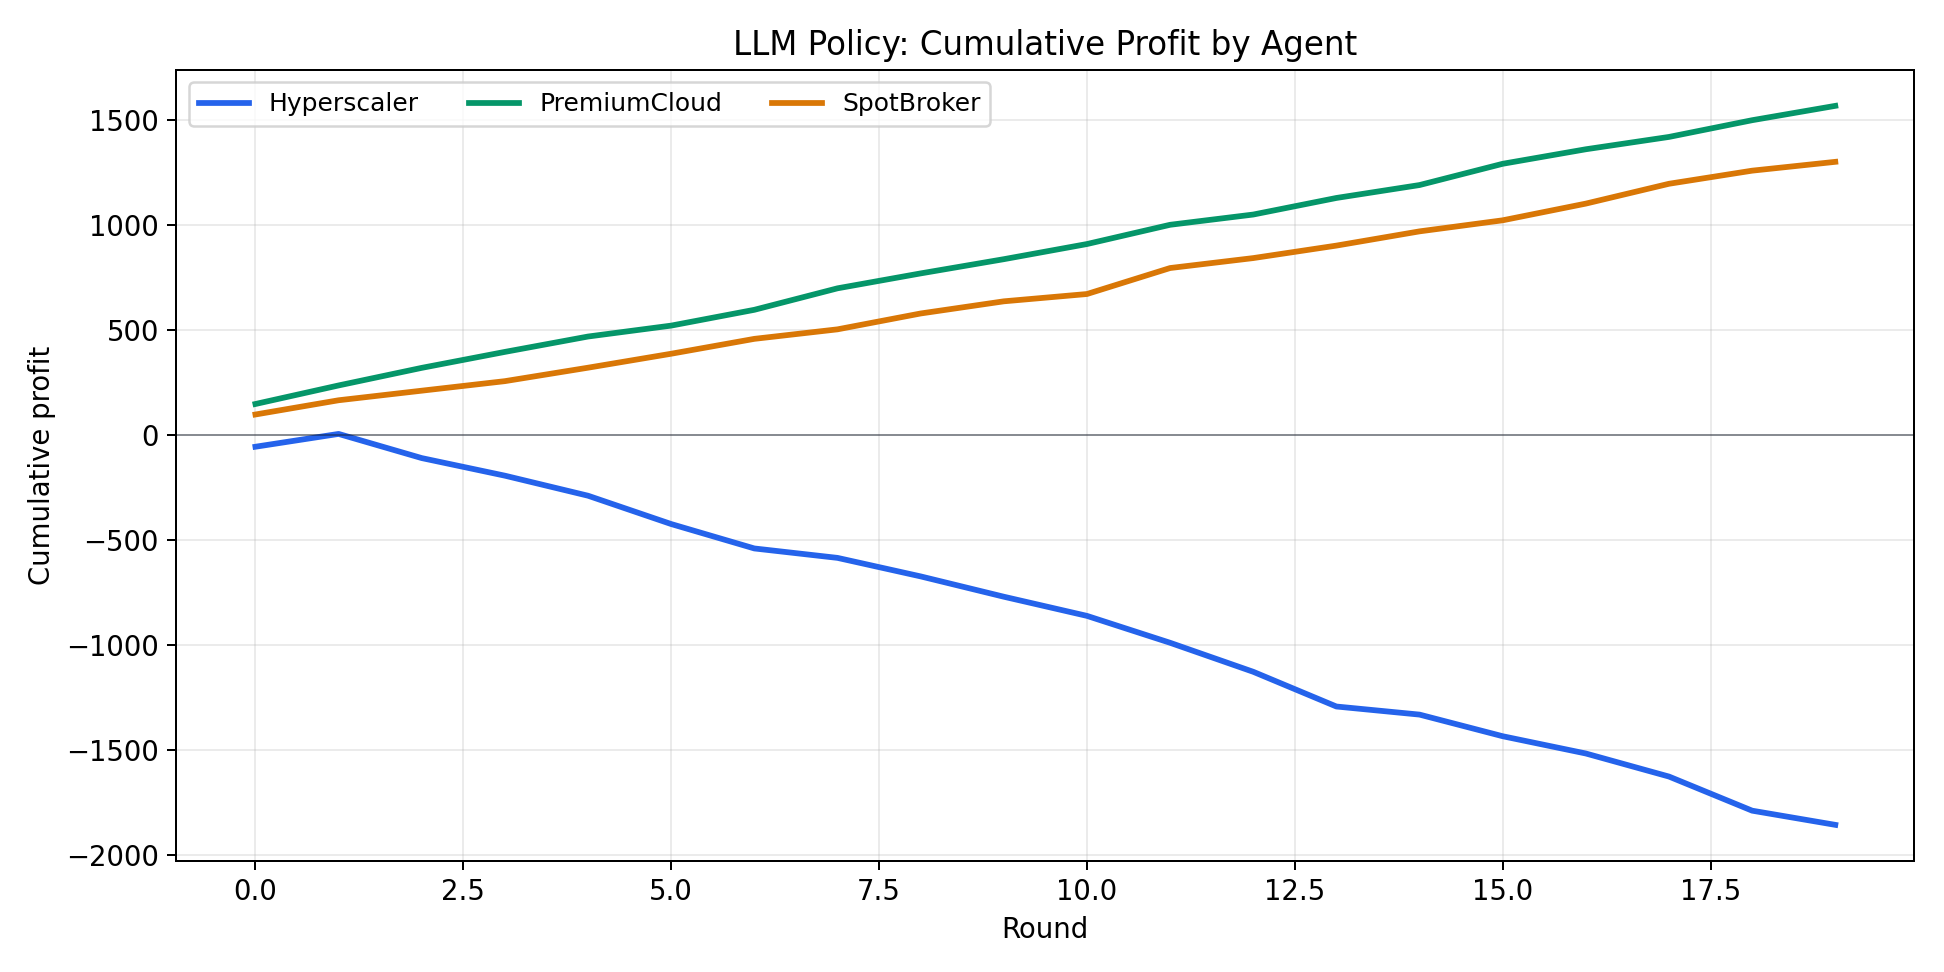
\includegraphics[width=0.82\textwidth]{figures/llm_profit_evolution.png}
\caption{LLM 策略下三个 Agent 的累计收益演化}\label{fig:llm-profit}
\end{figure}

图~\ref{fig:llm-profit} 显示，Hyperscaler 在早期即进入负收益区间，且亏损随轮次持续扩大；PremiumCloud 和 SpotBroker 则稳定积累正收益。这一结果说明，价格战并不必然带来长期优势，声誉和价格纪律在重复博弈中能够转化为稳定收益。

\subsection{履约、价格与状态演化}

\begin{figure}[H]
\centering
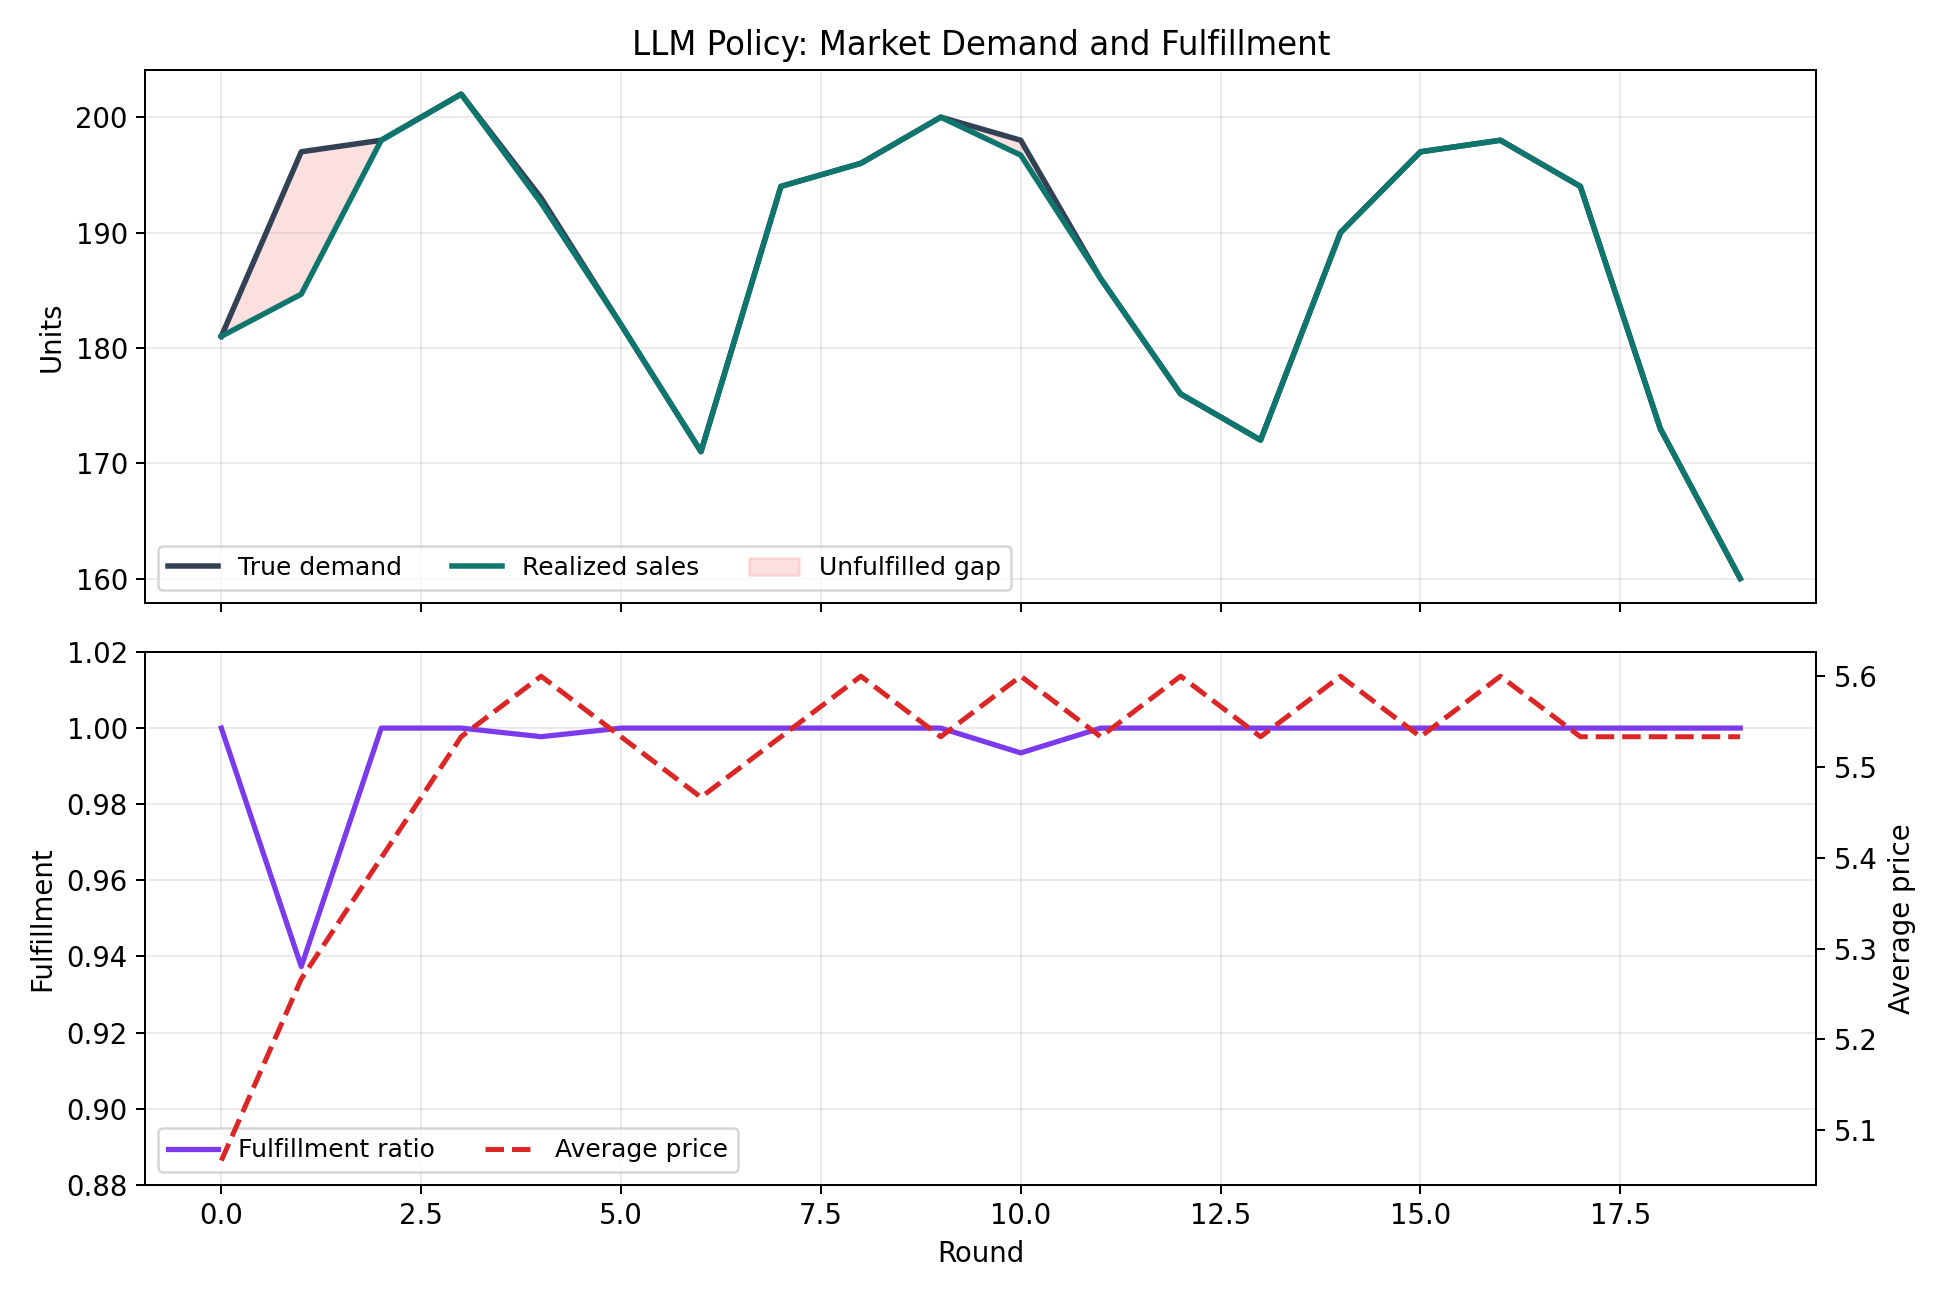
\includegraphics[width=0.82\textwidth]{figures/llm_market_fulfillment.png}
\caption{LLM 策略下市场需求、实现交付与平均价格}\label{fig:llm-fulfillment}
\end{figure}

图~\ref{fig:llm-fulfillment} 表明，LLM 策略下市场整体履约率维持在较高水平，未履约缺口主要集中在少数轮次。平均价格保持在较高区间，说明 LLM 并未简单地将所有 Agent 推向低价竞争，而是保留了角色差异。

\begin{figure}[H]
\centering
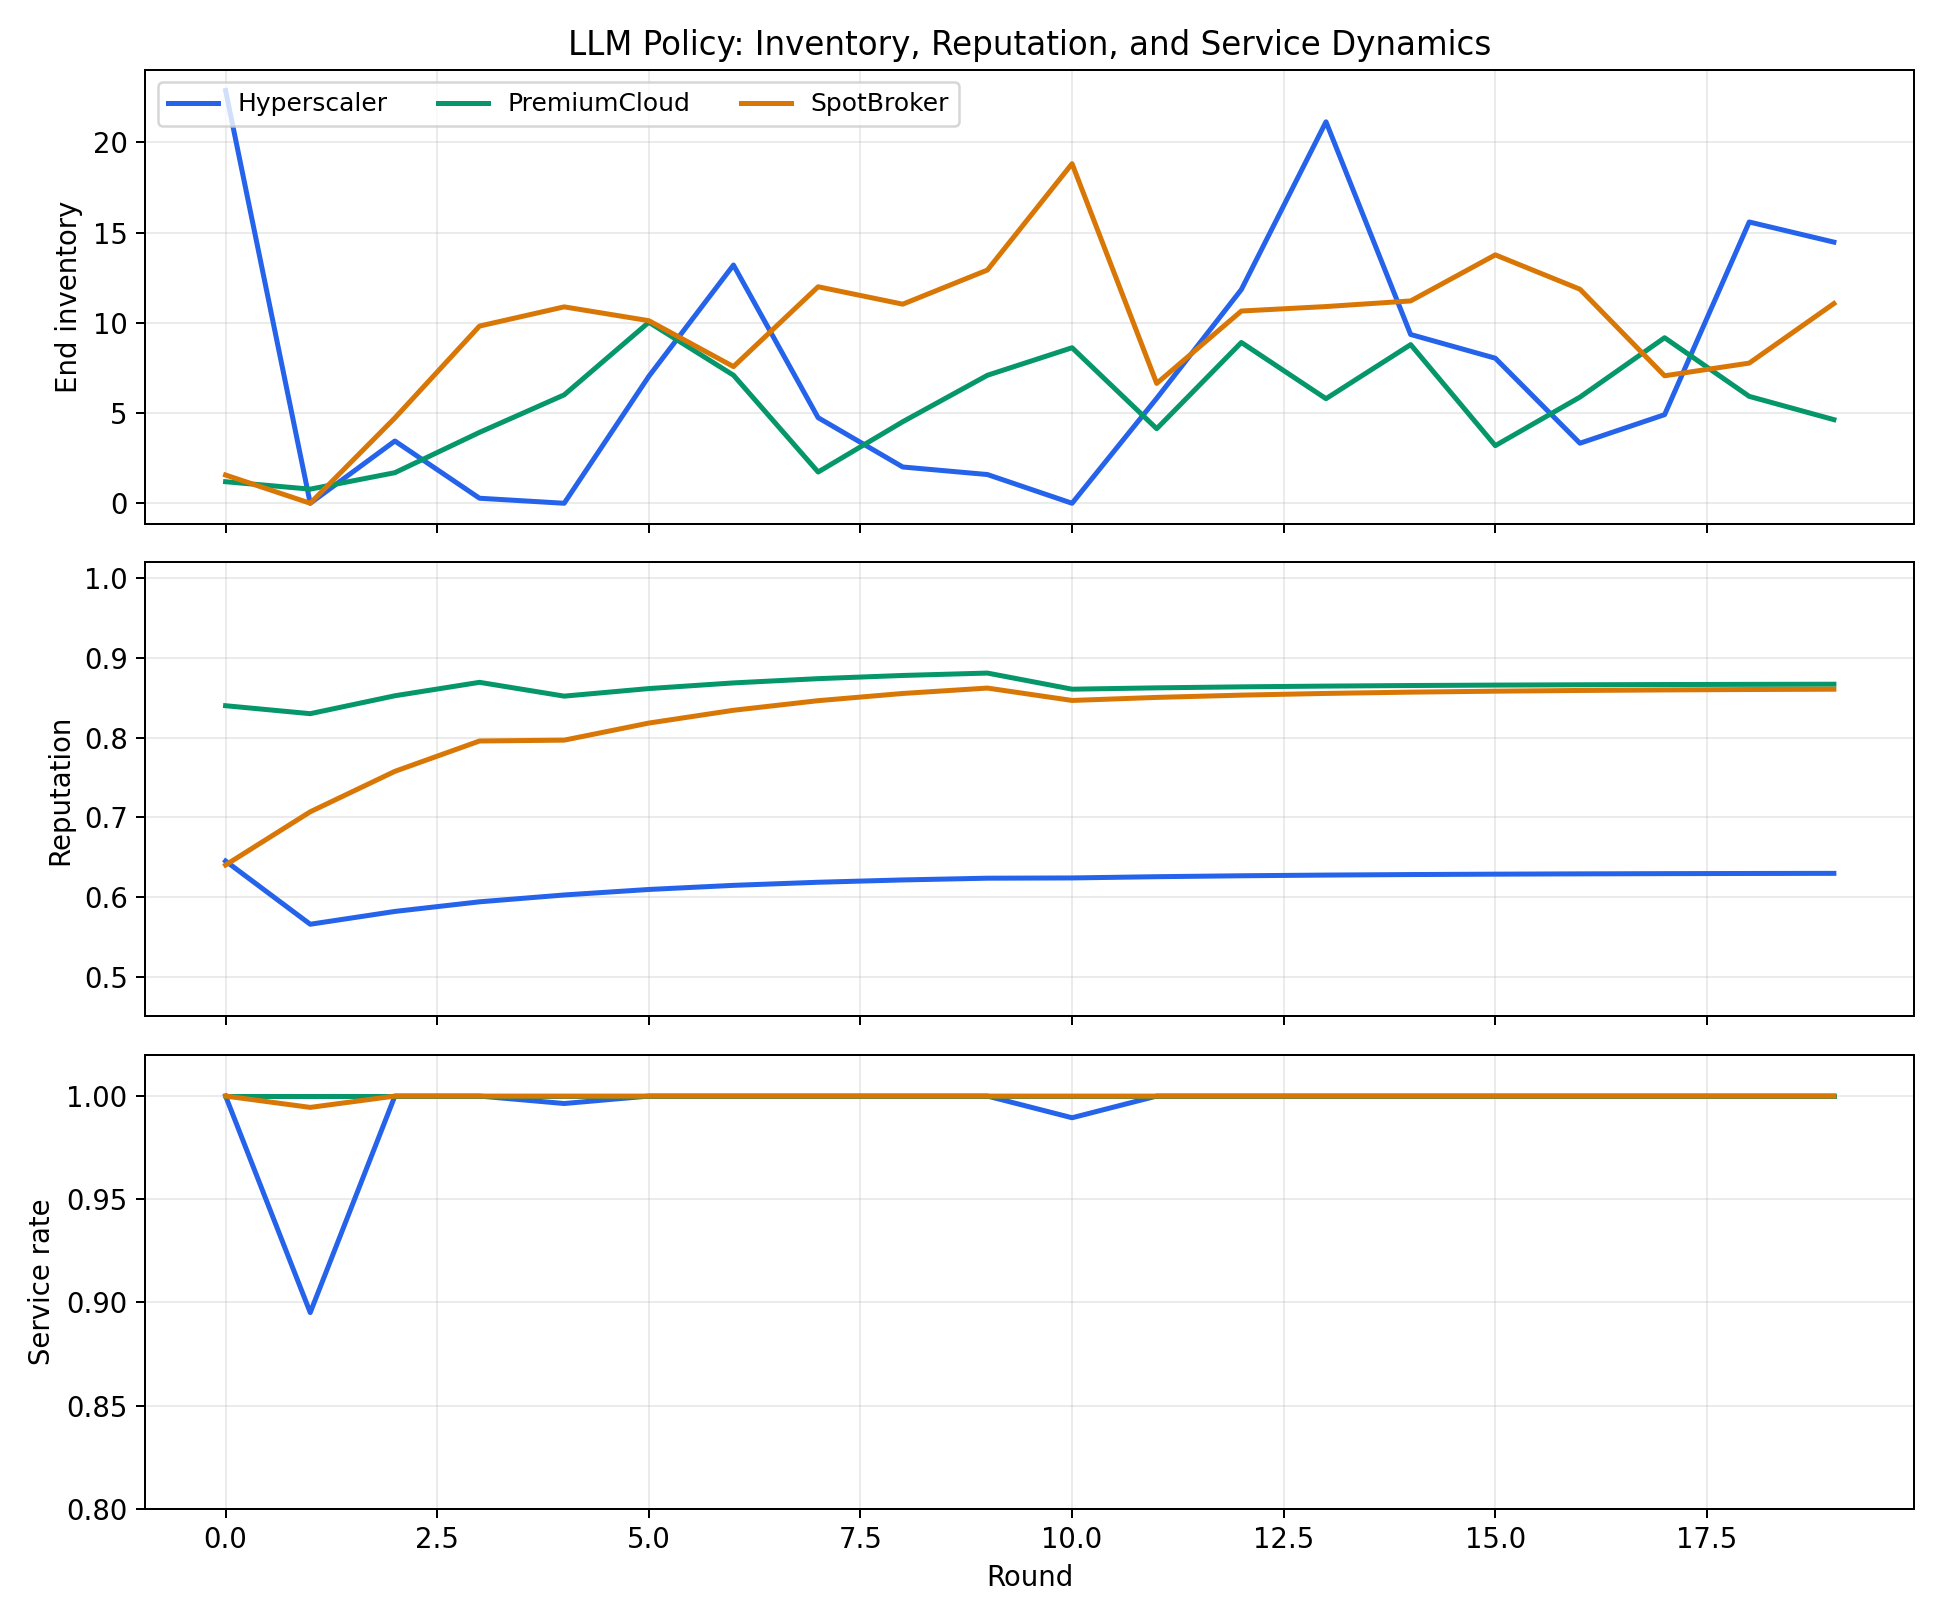
\includegraphics[width=0.82\textwidth]{figures/llm_agent_state_dynamics.png}
\caption{LLM 策略下库存、声誉和服务率动态}\label{fig:llm-state}
\end{figure}

图~\ref{fig:llm-state} 进一步展示了库存与声誉的动态。PremiumCloud 的声誉最稳，SpotBroker 保持中高声誉，Hyperscaler 则因持续低价和一次 default 事件受到声誉约束。库存层面，三者均未出现严重终局积压，这说明 RiskGate 和环境中的库存折旧成本对供给决策产生了约束。

\subsection{LLM 与启发式基线对照}

同 seed、同 20 轮设置下，LLM 策略与启发式策略的市场级结果见表~\ref{tab:llm-vs-heuristic}。

\begin{table}[H]
\centering
\caption{LLM 与启发式基线对照（20 轮，seed=7）}\label{tab:llm-vs-heuristic}
\vspace{0.3em}
\begin{tabular}{@{}lrrrr@{}}
\toprule
策略 & 市场总利润 & 履约率 & 平均声誉 & 总缺货 \\
\midrule
Heuristic & 763.91 & 0.9989 & 0.7836 & 3.95 \\
LLM & 1010.34 & 0.9963 & 0.7680 & 14.07 \\
\bottomrule
\end{tabular}
\end{table}

\begin{figure}[H]
\centering
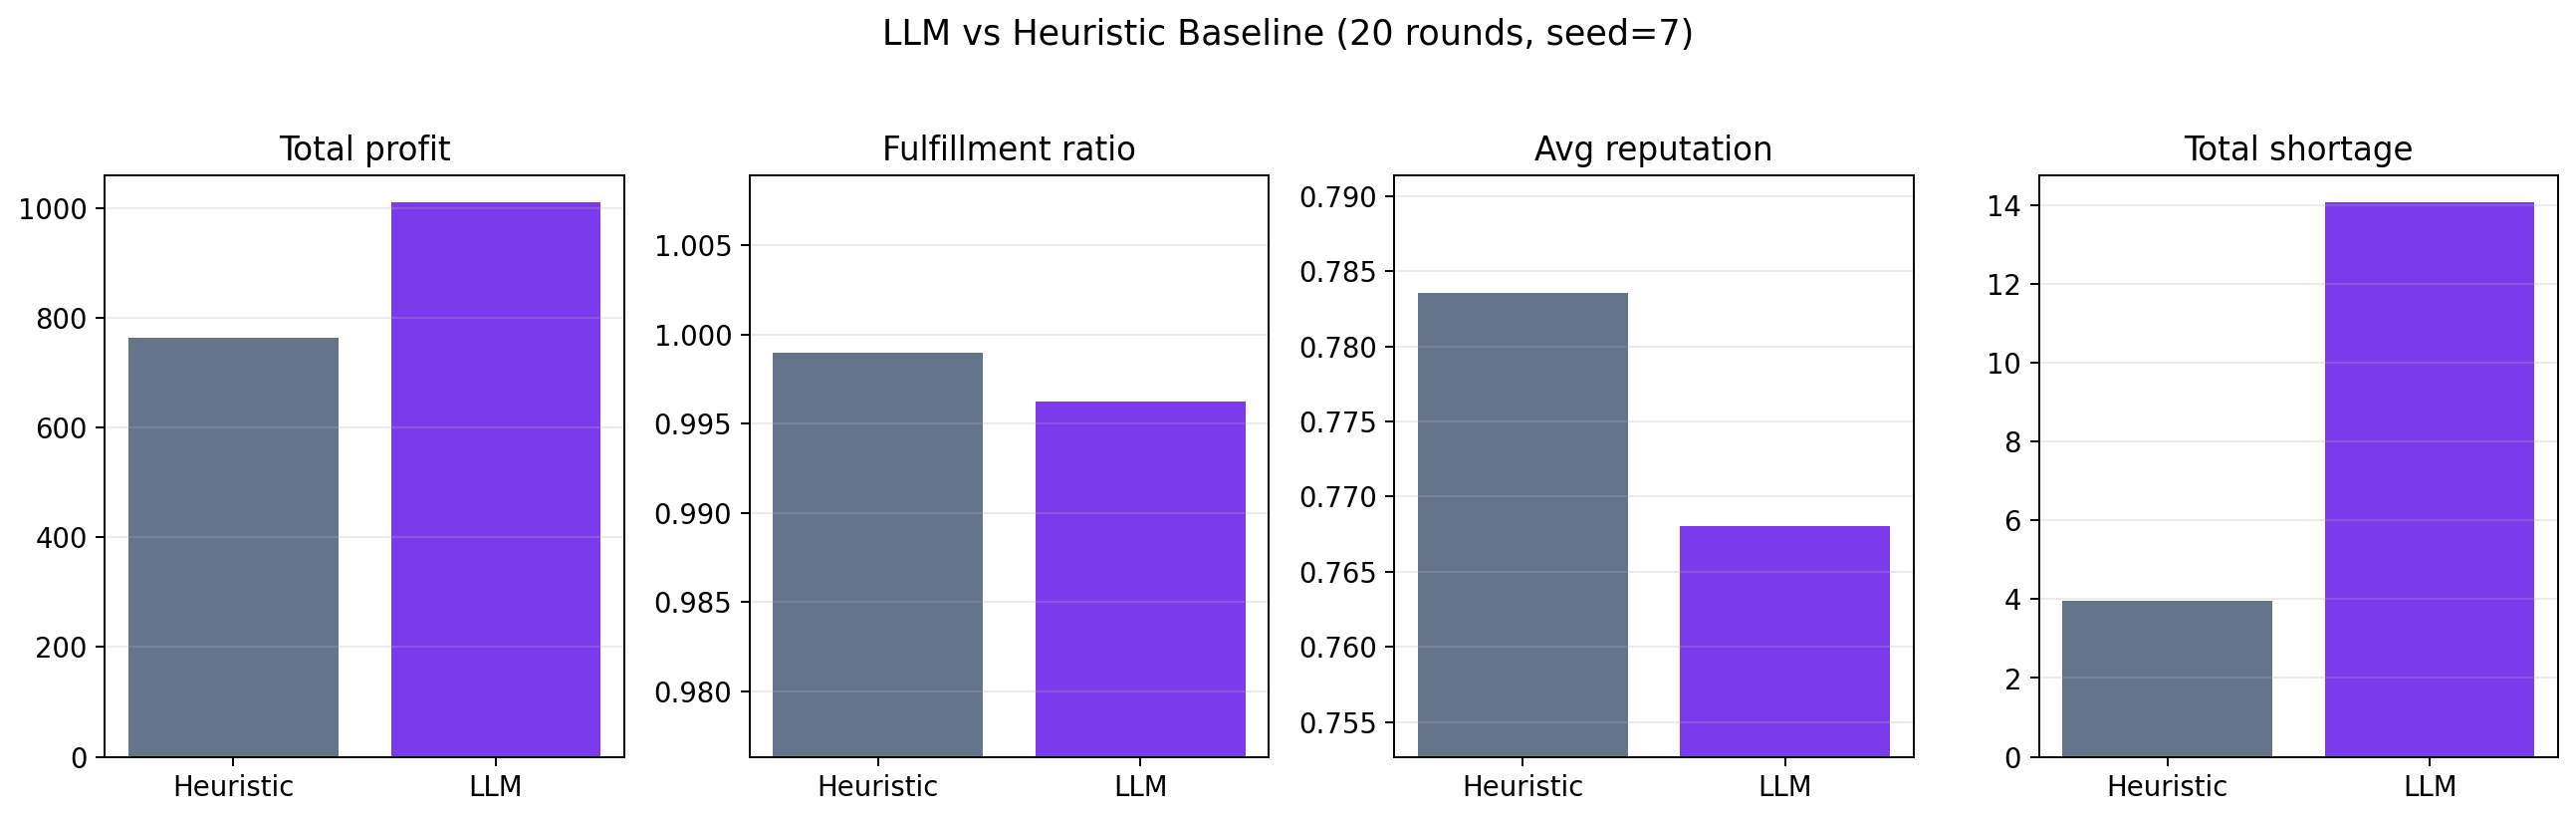
\includegraphics[width=0.92\textwidth]{figures/llm_vs_heuristic.png}
\caption{LLM 与启发式基线的市场级指标对照}\label{fig:llm-vs-heuristic}
\end{figure}

从表~\ref{tab:llm-vs-heuristic} 和图~\ref{fig:llm-vs-heuristic} 可以看到，LLM 策略的市场总利润高于 heuristic，但履约率略低、总缺货更高。这说明 LLM 决策在当前设置下更倾向于维持高价值订单和价格纪律，而不是机械追求最高履约率。该结果具有一定研究价值：LLM Agent 并非简单复制启发式规则，而是在角色 prompt、市场观察和风险约束共同作用下形成了不同的利润--服务权衡。

需要注意的是，当前 LLM 对照只完成了单 seed 实验。由于本地模型端点推理耗时较长，多 seed 长跑将在后续阶段继续补充，以判断该差异是否稳健。

%=============================================
\section{当前完成度}

截至中期，项目已经完成以下工作：

\begin{enumerate}
    \item 完成高端 GPU 算力现货与供应链博弈场景设计；
    \item 实现动态需求生成、需求分配、同行拆借、库存折旧、SLA 罚金和声誉更新；
    \item 实现三类异质 Agent，并拆分为 Forecaster、Pricer、Allocator 和 RiskGate 四阶段；
    \item 接入 OpenAI-compatible LLM 后端，并实现 JSON 输出解析和 heuristic fallback；
    \item 实现 CLI、本地 dashboard、CSV 输出、PDF 图表和 HTML 可视化；
    \item 实现 \texttt{quant/} 实验层，用于 benchmark、敏感性分析和报告导出；
    \item 完成 LLM 20 轮主实验和同 seed 启发式对照实验；
    \item 当前自动化测试集通过，共 27 个测试。
\end{enumerate}

从中期验收角度看，项目已经具备可运行、可复现、可解释、可视化和可扩展的核心能力。尤其是 LLM 模式已经不再停留于接口设计，而是能够完整参与多轮市场决策并产生可分析结果。

%=============================================
\section{问题与后续计划}

当前主要问题包括：

\begin{itemize}
    \item LLM 长轮次实验耗时较高，受本地 OpenAI-compatible 端点吞吐影响明显；
    \item 当前 LLM 结果仍以单 seed 为主，多 seed 稳健性尚未充分验证；
    \item Agent 阶段逻辑虽已拆分，但实现仍集中在 \texttt{agents.py}，后续应进一步模块化；
    \item 目前对 LLM 决策理由的记录还不够丰富，后续可保存每轮 prompt、raw response 和 fallback 标记；
    \item 还需要系统完成 ablation 实验，例如关闭声誉机制、关闭拆借机制或改变库存折旧强度。
\end{itemize}

后续计划分为三步。第一，扩展 LLM 实验规模，至少完成多 seed、不同需求冲击强度和不同声誉权重下的 LLM 对照。第二，完善报告层，自动生成论文所需的表格、图和统计摘要。第三，继续重构 Agent 模块，将阶段策略、LLM provider、prompt 模板和风险门控拆为更清晰的文件结构。

%=============================================
\section{结论}

本项目中期阶段已经完成从市场博弈设想到可运行 LLM 多 Agent 仿真平台的转化。系统能够模拟高端 GPU 算力市场中的动态需求、价格竞争、库存折旧、SLA 缺货、同行拆借和声誉演化，并能使用本地 LLM 后端直接生成 Agent 决策。

LLM 20 轮实验表明，三个 Agent 在相同市场环境中形成了明显分化：Hyperscaler 因持续低价竞争出现负利润，PremiumCloud 借助高声誉和价格纪律获得最高收益，SpotBroker 以灵活策略获得稳健正收益。与启发式基线相比，LLM 策略获得更高市场总利润，但承担了略高缺货风险。这说明 LLM Agent 在重复博弈中能够呈现不同于固定启发式规则的权衡行为，为后续研究 LLM 决策风格、声誉机制和市场稳定性提供了实验基础。

\section*{参考文献}
\begin{enumerate}
    \item Russell S., Norvig P. \textit{Artificial Intelligence: A Modern Approach}. Pearson, 2021.
    \item Shoham Y., Leyton-Brown K. \textit{Multiagent Systems: Algorithmic, Game-Theoretic, and Logical Foundations}. Cambridge University Press, 2008.
    \item Sutton R. S., Barto A. G. \textit{Reinforcement Learning: An Introduction}. MIT Press, 2018.
    \item Brown T. et al. Language Models are Few-Shot Learners. \textit{NeurIPS}, 2020.
    \item OpenAI. OpenAI-compatible Chat Completions API documentation.
\end{enumerate}

\end{document}
